% Options for packages loaded elsewhere
\PassOptionsToPackage{unicode}{hyperref}
\PassOptionsToPackage{hyphens}{url}
\PassOptionsToPackage{dvipsnames,svgnames,x11names}{xcolor}
%
\documentclass[
  11pt,
  a4paper,
]{article}
\usepackage{amsmath,amssymb}
\usepackage{setspace}
\usepackage{iftex}
\ifPDFTeX
  \usepackage[T1]{fontenc}
  \usepackage[utf8]{inputenc}
  \usepackage{textcomp} % provide euro and other symbols
\else % if luatex or xetex
  \usepackage{unicode-math} % this also loads fontspec
  \defaultfontfeatures{Scale=MatchLowercase}
  \defaultfontfeatures[\rmfamily]{Ligatures=TeX,Scale=1}
\fi
\usepackage[]{mathpazo}
\ifPDFTeX\else
  % xetex/luatex font selection
\fi
% Use upquote if available, for straight quotes in verbatim environments
\IfFileExists{upquote.sty}{\usepackage{upquote}}{}
\IfFileExists{microtype.sty}{% use microtype if available
  \usepackage[]{microtype}
  \UseMicrotypeSet[protrusion]{basicmath} % disable protrusion for tt fonts
}{}
\makeatletter
\@ifundefined{KOMAClassName}{% if non-KOMA class
  \IfFileExists{parskip.sty}{%
    \usepackage{parskip}
  }{% else
    \setlength{\parindent}{0pt}
    \setlength{\parskip}{6pt plus 2pt minus 1pt}}
}{% if KOMA class
  \KOMAoptions{parskip=half}}
\makeatother
\usepackage{xcolor}
\usepackage[margin=1in]{geometry}
\usepackage{longtable,booktabs,array}
\usepackage{calc} % for calculating minipage widths
% Correct order of tables after \paragraph or \subparagraph
\usepackage{etoolbox}
\makeatletter
\patchcmd\longtable{\par}{\if@noskipsec\mbox{}\fi\par}{}{}
\makeatother
% Allow footnotes in longtable head/foot
\IfFileExists{footnotehyper.sty}{\usepackage{footnotehyper}}{\usepackage{footnote}}
\makesavenoteenv{longtable}
\usepackage{graphicx}
\makeatletter
\def\maxwidth{\ifdim\Gin@nat@width>\linewidth\linewidth\else\Gin@nat@width\fi}
\def\maxheight{\ifdim\Gin@nat@height>\textheight\textheight\else\Gin@nat@height\fi}
\makeatother
% Scale images if necessary, so that they will not overflow the page
% margins by default, and it is still possible to overwrite the defaults
% using explicit options in \includegraphics[width, height, ...]{}
\setkeys{Gin}{width=\maxwidth,height=\maxheight,keepaspectratio}
% Set default figure placement to htbp
\makeatletter
\def\fps@figure{htbp}
\makeatother
\setlength{\emergencystretch}{3em} % prevent overfull lines
\providecommand{\tightlist}{%
  \setlength{\itemsep}{0pt}\setlength{\parskip}{0pt}}
\setcounter{secnumdepth}{-\maxdimen} % remove section numbering
\pagestyle{plain}
% definitions for citeproc citations
\NewDocumentCommand\citeproctext{}{}
\NewDocumentCommand\citeproc{mm}{%
  \begingroup\def\citeproctext{#2}\cite{#1}\endgroup}
\makeatletter
 % allow citations to break across lines
 \let\@cite@ofmt\@firstofone
 % avoid brackets around text for \cite:
 \def\@biblabel#1{}
 \def\@cite#1#2{{#1\if@tempswa , #2\fi}}
\makeatother
\newlength{\cslhangindent}
\setlength{\cslhangindent}{1.5em}
\newlength{\csllabelwidth}
\setlength{\csllabelwidth}{3em}
\newenvironment{CSLReferences}[2] % #1 hanging-indent, #2 entry-spacing
 {\begin{list}{}{%
  \setlength{\itemindent}{0pt}
  \setlength{\leftmargin}{0pt}
  \setlength{\parsep}{0pt}
  % turn on hanging indent if param 1 is 1
  \ifodd #1
   \setlength{\leftmargin}{\cslhangindent}
   \setlength{\itemindent}{-1\cslhangindent}
  \fi
  % set entry spacing
  \setlength{\itemsep}{#2\baselineskip}}}
 {\end{list}}
\usepackage{calc}
\newcommand{\CSLBlock}[1]{\hfill\break\parbox[t]{\linewidth}{\strut\ignorespaces#1\strut}}
\newcommand{\CSLLeftMargin}[1]{\parbox[t]{\csllabelwidth}{\strut#1\strut}}
\newcommand{\CSLRightInline}[1]{\parbox[t]{\linewidth - \csllabelwidth}{\strut#1\strut}}
\newcommand{\CSLIndent}[1]{\hspace{\cslhangindent}#1}
\usepackage{lineno} % add 
\usepackage{amsmath} % add 
\linenumbers % turns line numbering on 

% Allowing for landscape pages
\usepackage{lscape}
\newcommand{\blandscape}{\begin{landscape}}
\newcommand{\elandscape}{\end{landscape}}

% Left justification of the text: see https://www.sharelatex.com/learn/Text_alignment
% \usepackage[document]{ragged2e} % already in the latex template
\newcommand{\bleft}{\begin{flushleft}}
\newcommand{\eleft}{\end{flushleft}}


% Add Supplementary Tables and Figures
% Code from https://stackoverflow.com/a/51337664
\newcommand{\beginsupplement}{
  \setcounter{table}{0}  
  \renewcommand{\thetable}{S\arabic{table}}
  \setcounter{figure}{0} 
  \renewcommand{\thefigure}{S\arabic{figure}}
}



\ifLuaTeX
  \usepackage{selnolig}  % disable illegal ligatures
\fi
\usepackage{bookmark}
\IfFileExists{xurl.sty}{\usepackage{xurl}}{} % add URL line breaks if available
\urlstyle{same}
\hypersetup{
  pdftitle={Estimating coypu (Myocastor coypus) abundance using removal data},
  pdfauthor={Olivier Gimenez1*},
  colorlinks=true,
  linkcolor={RoyalBlue},
  filecolor={Maroon},
  citecolor={Blue},
  urlcolor={RoyalBlue},
  pdfcreator={LaTeX via pandoc}}

\title{Estimating coypu (Myocastor coypus) abundance using removal data}
\author{Olivier Gimenez\textsuperscript{1}*}
\date{2024-12-25}

\begin{document}
\maketitle

\setstretch{2}
\small

\textsuperscript{1} CEFE, Univ Montpellier, CNRS, EPHE, IRD, Montpellier, France

\texttt{*} Corresponding author: \href{mailto:olivier.gimenez@cefe.cnrs.fr}{\nolinkurl{olivier.gimenez@cefe.cnrs.fr}}

\normalsize

\vspace{1cm}
\hrule

blabla.

\vspace{3mm}
\hrule
\vspace{5mm}

\emph{Keywords}: Invasive species, Multinomial N-mixture, Population size, Statistical ecology

\bleft
\newpage

\section{Introduction}\label{introduction}

Invasive species are a significant global issue, with wide-ranging impacts on ecosystems, economies, and public health (\citeproc{ref-Petr2020}{Pyšek et al. 2020}, \citeproc{ref-Roy2024}{Roy et al. 2024}). Among these, the financial, epidemiological, social, and ecological costs associated with invasive rodents are substantial, as they damage infrastructures, degrade agricultural systems, and act as reservoirs for zoonotic diseases (\citeproc{ref-Diagne2023}{Diagne et al. 2023}).

Effective management of invasive species requires the estimation of population abundance for guiding control efforts and evaluating the success of eradication or regulation programs (\citeproc{ref-Williams2002}{Williams et al. 2002}, \citeproc{ref-Thompson2021}{Thompson et al. 2021}). However, the challenge in estimating animal abundance is that individuals are not always observed even when present due to imperfect detection (\citeproc{ref-Borchers2002}{Borchers et al. 2002}, \citeproc{ref-Seber2023}{Seber and Schofield 2023}). Ignoring imperfect detection leads to biased estimates of population abundance (\citeproc{ref-Kery2008}{Kéry and Schmidt 2008}). To account for imperfect detection, capture-recapture methods are usually used to correct observed counts (\citeproc{ref-Mccrea2015}{McCrea and Morgan 2015}). Yet, for invasive species, capture-recapture is often impractical, as ethical and management concerns typically prevent the release of captured animals.

An alternative approach involves the use of removal methods (\citeproc{ref-Rodriguez2021}{Rodriguez de Rivera and McCrea 2021}) in which individuals are captured and permanently removed from the study area during successive sampling occasions. This process leads to a decrease in the expected number of captures by a consistent proportion over time (rather than by a fixed amount decline), which informs on the total abundance as the initial population determines how quickly the number of individuals available for capture diminishes.

While standard removal methods are well-established (\citeproc{ref-Moran1951}{Moran 1951}, \citeproc{ref-Zippin1956}{Zippin 1956}, \citeproc{ref-Zippin1958}{1958}, \citeproc{ref-Rodriguez2021}{Rodriguez de Rivera and McCrea 2021}), recent advances in population ecology are still underutilized in the context of invasive species. Hierarchical models in particular ont percé (\citeproc{ref-RD2008}{Royle and Dorazio 2008}, \citeproc{ref-KR2015}{Kéry and Royle 2015}) comme ils permettent de i) séparer clairement/formellent the biological processes of interest (e.g., population dynamics) from observation processes (e.g., imperfect detection) et donc d'aider à bien modéliser, et ii) allow the inclusion of environmental, spatial, or temporal covariates at multiple levels to explore how different factors influence ecological processes, iii) by modeling parameters hierarchically, information can be shared across groups or regions, improving estimates for smaller datasets (known as ``partial pooling'' and random effects). This is especially useful when some groups have limited data but still share common characteristics with others.

While standard removal methods are well-established (\citeproc{ref-Moran1951}{Moran 1951}, \citeproc{ref-Zippin1956}{Zippin 1956}, \citeproc{ref-Zippin1958}{1958}, \citeproc{ref-Rodriguez2021}{Rodriguez de Rivera and McCrea 2021}), recent advances in population ecology remain underutilized in the context of invasive species. Hierarchical models, in particular, have gained tractino (\citeproc{ref-RD2008}{Royle and Dorazio 2008}, \citeproc{ref-KR2015}{Kéry and Royle 2015}) due to their ability to: (i) explicitly separate biological processes of interest (e.g., population dynamics) from observation processes (e.g., imperfect detection), thus enabling more accurate modeling; (ii) incorporate environmental, spatial, or temporal covariates at multiple levels, allowing exploration of how various factors influence ecological processes; and (iii) share information across groups by modeling parameters hierarchically with random effects, which improves estimates for groups with fewer data.

In this paper, I showcase the application of a hierarchical formulation of removal models, the multinomial N-mixture model (\citeproc{ref-Dorazio2005}{Dorazio et al. 2005}), to estimate the abundance of an invasive coypu (\emph{Myocastor coypus}) population in southern France. Coypu, a rodent native to South America, has established widespread invasive populations in France, where it causes extensive damage to infrastructure and crops and acts as a healthy carrier of leptospirosis, a potentially serious zoonotic disease (\citeproc{ref-Bonnet2021}{Bonnet et al. 2021}, \citeproc{ref-Bonnet2023}{2023}). Using removal data, I demonstrate the implementation of the multinomial N-mixture model to estimate coypu abundance, exploring both frequentist and Bayesian approaches. Furthermore, I investigate how detection probabilities and abundance are influenced by habitat and climatic factors. Finally, I conduct a simulation study to evaluate the performance of the multinomial N-mixture model under varying numbers of sampling sites and occasions.

\section{Methods}\label{methods}

\subsection{Multinomial N-mixture model}\label{multinomial-n-mixture-model}

Think of a die with six sides. The die has a 1 in 6 chance of landing on face 1, the same for face 2, and so on. If I roll the die 30 times, I expect to get face 1 five times, face 2 five times, and so on, on average. In this experiment, \(y_1\), the vector made of the number of 1s, \(y_2\), the number of 2s, \(\ldots\), and \(y_6\), the number of 6s, follows a multinomial distribution with parameters the number of rolls (30) and probabilities \((1/6, 1/6, ..., 1/6)\).

Now think of a removal campaign conducted over 3 months. We record the number of coypu \(y_1\) captured in month 1, \(y_2\) in month 2, \(y_3\) in month 3, and let \(y_4\) represent the number of coypu never captured. Let \(p\) be the probability of capturing a coypu in a given month. The probability of capturing a coypu in the first month is \(\pi_1 = p\). The probability of capturing a coypu in the second month is \(\pi_2 = (1-p)p\) the probability of not capturing it in the first month \((1 - p)\) multiplied by the probability of capturing it in the second month \(p\). The probability of capturing a coypu in the third month is \(\pi_3 = (1-p)(1-p)p\), the probability of not capturing it in the first and second months, \((1 - p)(1 - p)\), multiplied by the probability of capturing it in the third month, \(p\). Finally, the probability of never being captured is \(\pi_4 = 1 - (p + (1-p)p + (1-p)(1-p)p)\) the complement of the probability of being captured in the first, second, or third month.

If we assume that \(N\) represents the abundance, then we have that the vector of counts \((y_1, y_2, y_3, y_4)\) follows a multinomial distribution with parameters \(N\) and probabilities \((\pi_1,\pi_2,\pi_3,\pi_4)\). INTRODUCE \(N \sim \text{Poisson}(\lambda)\). AND NEGATIVE BINOMIAL. ALSO SEVERAL SITES. EXPLAIN LA PARTIE HIERARCHIQUE ICI. METTRE UN EFFET ALEATOIRE QUELQUE PART?

FAIRE LE LIEN ENTRE LE DE ET LA CAMPAGNE DE PIEGEAGE.

Parameters \(N\), \(p\), and \(\lambda\) are unknown and need to be estimated. In a frequentist framework, marginalization is performed by summing over all possible values of \(N\). In a Bayesian framework, all these parameters are estimated directly, which simplifies the process.

Both parameters, \(N\) and \(p\), can be modeled as functions of explanatory spatial variables, in the spirit of generalized linear models, and logistic regressions for example.

Citer chapitre dans bouquin de Kéry and Royle qui va bien (vol I).

\subsection{Implementation}\label{implementation}

For all analyses, I used the statistical language \texttt{R} (\citeproc{ref-R_Core_Team_2024}{R Core Team 2024}). I used the \texttt{tidyverse} (\citeproc{ref-Wickham_2019}{Wickham et al. 2019}) suite of packages for data manipulation and visualization and \texttt{sf} (\citeproc{ref-Pebesma_2023}{Pebesma and Bivand 2023}) for dealing with spatial data. I fitted models within the frequentist framework\ldots{} unmarked (\citeproc{ref-Kellner_2023}{Kellner et al. 2023}). Bayesian framework using the \texttt{ubms} (\citeproc{ref-Kellner_2021}{Kellner et al. 2021}) package. I specified weakly informative priors for all parameters, specifically normal distributions with mean 0 and standard deviation 1.5 for regression parameters, and uniform distributions for the partial sill, range parameter and detection probability. I ran two chains for a total of 15,000 iterations with a burn-in of 5,000 iterations. I summarized posterior distributions with posterior mean and 95\% credible intervals. I assessed model convergence using R-hat values (\textless{} 1.1), effective sample size (\textgreater{} 100), and visual inspection of the trace plots.

\section{Simulations}\label{simulations}

Voir un peu comment se comporte le modèle en fonction du nombre de sites et d'occasions.

I conducted a simulation study to evaluate model performance by examining parameter bias and prediction error. I simulated a stream network over \(S = 100\) sites using an exponential tail-down structure (inspired by the case study, see previous section) with partial sill \(\sigma^2 = 2\) and range parameter \(\theta = 10\). I considered a single covariate, normally distributed with mean 0 and standard deviation 1, with a linear effect (on the logit scale) on the occupancy probability with intercept \(\beta_0 = 0.5\) and slope \(\beta_1 = 1\). I simulated the observation process with a detection probability \(p = 0.6\) across 5 repeated visits per site. I fitted both models, with and without spatial autocorrelation, to the simulated data, and I repeated this procedure 100 times. Eventually, I calculated the relative bias for each parameter and the root mean square prediction error (RMSPE) for each model. Unmarked only to speed up process.

\section{Case studies}\label{case-studies}

Temperature. Citer krigR. Month effect. First case study for hierarchical and covariates. Second case study for random effect.

\subsection{Coypus in France}\label{coypus-in-france}

Tableau avec les données. Et les covariables.

To illustrate the approach, I investigated the impact of human disturbance on the occupancy of European otter (\emph{Lutra lutra}) in France. The otter, a semi-aquatic mammal, faced near extinction in the 20th century in France due to extensive hunting for its fur. With hunting bans and protection efforts, the species is now recolonizing the country, and the ecological question is assessing its current distribution. Data on otter detection and non-detection were collected in 2003-2005 in the Midi-Pyrénées region. Observers searched for signs of otter presence at a small river catchment scale, which was used as the spatial sampling unit.

\subsection{Muskrats in the Netherlands}\label{muskrats-in-the-netherlands}

Pour muskrats: \url{https://ipt.nlbif.nl/resource?r=hwh_muskrat_1987-2014\#anchor-versions} and \url{https://www.gbif.org/dataset/7d75109d-a6cb-4e90-89d0-79d08577c580}.

\section{Results and discussion}\label{results-and-discussion}

The results of the simulation study underscored the importance of accounting for spatial autocorrelation - see Fig. \ref{fig:bias}. Ignoring spatial autocorrelation led to a relative bias of -26\% in the slope of the covariate, compared to just 0.7\% when spatial autocorrelation was included. Although the range parameter exhibited substantial bias (330\%), this outcome was expected. In spatial models, there is typically a strong positive relationship between the range parameter and the partial sill (\citeproc{ref-zhang2004}{Zhang 2004}, \citeproc{ref-VerHoef2024}{Ver Hoef et al. 2024}), which showed a bias of 12\%. Importantly, the ratio of the range parameter to the partial sill can be reliably estimated (\citeproc{ref-zhang2004}{Zhang 2004}), as evidenced by its negligible bias (0.9\%). Overall, the root mean square prediction error (RMSPE) was lower for the model with spatial correlation (RMSPE = 0.18) compared to the model without it (RMSPE = 0.23).

Coypus case study. I provide the parameter estimates from the new model accommodating spatial autocorrelation , unless otherwise specified. Detection probability was less than one, estimated at 0.71 (0.59, 0.80), which justified the use of occupancy models. The proportion of cultivated area had no effect, with a slope estimated at 0.60 (-0.67, 1.96). Population density also had no effect on occupancy probability, with a slope estimated at -0.96 (-2.24, 0.17). However, I did find a negative effect when spatial autocorrelation was ignored, with a slope estimated at -1.10 (-1.99, -0.34). This latter result aligns with a previous analysis of a more extensive dataset (\citeproc{ref-Couturier2024}{Couturier et al. 2023}) that also ignored spatial autocorrelation.

Muskrats case study. - see Fig. \ref{fig:muskrats}

Two short-term perspectives arise from this work. From a methodological perspective, the new approach could be extended to multi-season occupancy models, enabling the modeling of colonization probability as a function of distance to habitat features that may impede species movement (e.g., \citeproc{ref-Kervellec2023}{Kervellec et al. 2024}). This would facilitate the quantification of landscape connectivity in freshwater ecosystems. Such development requires moving to spatio-temporal models for stream and river data, which have recently become avaible (\citeproc{ref-Santos2022}{Santos-Fernandez et al. 2022}). From an ecological perspective, the new approach presents significant potential for the analysis of environmental DNA (eDNA). The eDNA methodology offers substantial promise for the non-invasive monitoring of biodiversity in freshwater ecosystems (\citeproc{ref-Carraro2020}{Carraro et al. 2020}). While spatial stream network models have been employed to analyze eDNA data (\citeproc{ref-Winkowski2024}{Winkowski et al. 2024}), these models have overlooked the issue of imperfect detection. Previous studies have recognized occupancy models as effective tools for eDNA data analysis (\citeproc{ref-Burian2021}{Burian et al. 2021}), with some considering spatial autocorrelation (\citeproc{ref-Chen2019}{Chen and Ficetola 2019}), however they have yet to integrate spatial stream networks. The new approach addresses this gap by incorporating both imperfect detection and spatial stream networks.

Recommendation. Record effort, 0s from non-sampling and 0s for non-detections. Close-kin as alternative. Use for projections. Also multispecies (cf N-mixture multispecies). Also immigration et papers par d'autres sur multinomial N-mixture extensions. Here, just AR(1) as in Outhwaite et al. (\citeproc{ref-Outhwaite2018}{2018}) random walk, mais mechanisms et demog parameters possible. Effectifs en eux-memes un peu meaningless, boucle de gestion adaptative.

Two main assumptions: constant capture, closed pop.

Pb lack of fit. Main three are overdispersion, ok with negative binomial (give results); closure ok w/ open models w/ survival/recruitment or simple multisession (papier census aérien); spatial autocorrelation, ok en classique (GAM ou autre), et aussi possible w/ stream networks pour coypus; iv) Hierarchical models are well-suited for representing dependencies in space, time, or species interactions, which are common in ecological systems.

Pour ouvert, papier Eleni open (mais permanent emigration) (\citeproc{ref-Matechou2016}{Matechou et al. 2016}), puis Zhou pour temporary emigration (\citeproc{ref-Zhou2019}{Zhou et al. 2019}). Ajouter aussi le papier de Link pour dispersal (\citeproc{ref-Link2018}{Link et al. 2018}).

Un peu chiant unmarked. Avantage bayésien. No boundary estimates, easy random effects.

Difference entre population et species.

Les hypothèses du modèle. Ici ou en discussion. Population fermée: pas de naissances/morts ou émigration/immigration pendant la période de piégeage. Les sites de piégeage sont indépendants: les prélèvements sur un site n'affectent pas ceux faits sur un autre site.

Lack of fit, overdispersion and negative binomial.

Si random effect site pas pertinent, on peut faire du spatial autocorrelation avec RSR. Easy avec ubms, possible aussi avec NIMBLE (\url{https://wildlife.onlinelibrary.wiley.com/doi/10.1002/jwmg.22296}). Pas possible avec unmarked.

Pour l'ouvert, possible avec unmarked, pas ubms. OK avec NIMBLE.

Pour NB, pas possible avec ubms. OK avec NIMBLE et unmarked.

\section{Acknowledgments}\label{acknowledgments}

I would like to warmly thank X and Y for data.

\subsection{Data availability statement}\label{data-availability-statement}

Data and code are available at \href{https://github.com/oliviergimenez/counting-rodents}{https://github.com/oliviergimenez/counting-rodents}.

\subsection{Funding statement}\label{funding-statement}

Ici mettre financement UM.

\subsection{Conflict of interest disclosure}\label{conflict-of-interest-disclosure}

The author has no conflicts of interest to declare.

\section{References}\label{references}

\phantomsection\label{refs}
\begin{CSLReferences}{1}{0}
\bibitem[\citeproctext]{ref-Bonnet2023}
Bonnet, M., G. Guédon, S. Bertolino, C. Harmange, A. Pagano, D. Picard, and O. Pays. 2023. Improving the management of aquatic invasive alien rodents in france: Appraisal and recommended actions. Management of Biological Invasions 14:625--640.

\bibitem[\citeproctext]{ref-Bonnet2021}
Bonnet, M., G. Guédon, M. Pondaven, S. Bertolino, D. Padiolleau, V. Pénisson, F. Gastinel, F. Angot, P.-C. Renaud, A. Frémy, and O. Pays. 2021. Aquatic invasive alien rodents in western france: Where do we stand today after decades of control? Plos One 16:1--14.

\bibitem[\citeproctext]{ref-Borchers2002}
Borchers, D. L., S. T. Buckland, and Z. W. 2002. Estimating animal abundance: Closed populations. Springer-Verlag, London.

\bibitem[\citeproctext]{ref-Burian2021}
Burian, A., Q. Mauvisseau, M. Bulling, S. Domisch, S. Qian, and M. Sweet. 2021. Improving the reliability of eDNA data interpretation. Molecular Ecology Resources 21:1422--1433.

\bibitem[\citeproctext]{ref-Carraro2020}
Carraro, L., E. Mächler, R. Wüthrich, and F. Altermatt. 2020. Environmental DNA allows upscaling spatial patterns of biodiversity in freshwater ecosystems. Nature Communications 11:3585.

\bibitem[\citeproctext]{ref-Chen2019}
Chen, W., and G. F. Ficetola. 2019. Conditionally autoregressive models improve occupancy analyses of autocorrelated data: An example with environmental DNA. Molecular Ecology Resources 19:163--175.

\bibitem[\citeproctext]{ref-Couturier2024}
Couturier, T., J. Steinmetz, P. Defos du Rau, D. Marc, E. Trichet, R. Gomes, and A. Besnard. 2023. Intensive agriculture as the main limiting factor of the otter's return in southwest france. Biological Conservation 279:109927.

\bibitem[\citeproctext]{ref-Diagne2023}
Diagne, C., L. Ballesteros-Mejia, R. Cuthbert, T. Bodey, J. Fantle-Lepczyk, E. Angulo, A. Bang, G. D. G, and F. Courchamp. 2023. Economic costs of invasive rodents worldwide: The tip of the iceberg. PeerJ 11:e14935.

\bibitem[\citeproctext]{ref-Dorazio2005}
Dorazio, R. M., H. L. Jelks, and F. Jordan. 2005. Improving removal-based estimates of abundance by sampling a population of spatially distinct subpopulations. Biometrics 61:1093--1101.

\bibitem[\citeproctext]{ref-Kellner_2021}
Kellner, K. F., N. L. Fowler, T. R. Petroelje, T. M. Kautz, D. E. Beyer, and J. L. Belant. 2021. \href{https://doi.org/10.1111/2041-210X.13777}{{ubms}: An {R} package for fitting hierarchical occupancy and n-mixture abundance models in a bayesian framework}. Methods in Ecology and Evolution 13:577--584.

\bibitem[\citeproctext]{ref-Kellner_2023}
Kellner, K. F., A. D. Smith, J. A. Royle, M. Kery, J. L. Belant, and R. B. Chandler. 2023. \href{https://www.jstatsoft.org/v43/i10/}{The {unmarked} {R} package: Twelve years of advances in occurrence and abundance modelling in ecology}. Methods in Ecology and Evolution 14:1408--1415.

\bibitem[\citeproctext]{ref-Kervellec2023}
Kervellec, M., T. Couturier, S. Bauduin, D. Chenesseau, P. D. du Rau, N. Drouet-Hoguet, C. Duchamp, J. Steinmetz, J.-M. Vandel, and O. Gimenez. 2024. Bringing circuit theory into spatial occupancy models to assess landscape connectivity. Methods in Ecology and Evolution.

\bibitem[\citeproctext]{ref-KR2015}
Kéry, M., and J. A. Royle. 2015. Applied hierarchical modeling in ecology: Analysis of distribution, abundance and species richness in r and BUGS. Academic Press, London, UK.

\bibitem[\citeproctext]{ref-Kery2008}
Kéry, M., and B. Schmidt. 2008. Imperfect detection and its consequences for monitoring in conservation. Community Ecology 9:207--216.

\bibitem[\citeproctext]{ref-Link2018}
Link, W. A., S. J. Converse, A. A. Yackel Adams, and N. J. Hostetter. 2018. Analysis of population change and movement using robust design removal data. Journal of Agricultural, Biological and Environmental Statistics 23:463--477.

\bibitem[\citeproctext]{ref-Matechou2016}
Matechou, E., R. S. McCrea, B. J. T. Morgan, D. J. Nash, and R. A. Griffiths. 2016. {Open models for removal data}. The Annals of Applied Statistics 10:1572--1589.

\bibitem[\citeproctext]{ref-Mccrea2015}
McCrea, R. S., and B. J. T. Morgan. 2015. Analysis of capture-recapture data. Chapman \& Hall.

\bibitem[\citeproctext]{ref-Moran1951}
Moran, P. A. P. 1951. A mathematical theory of animal trapping. Biometrika 38:307--311.

\bibitem[\citeproctext]{ref-Outhwaite2018}
Outhwaite, C. L., R. E. Chandler, G. D. Powney, B. Collen, R. D. Gregory, and N. J. B. Isaac. 2018. Prior specification in bayesian occupancy modelling improves analysis of species occurrence data. Ecological Indicators 93:333--343.

\bibitem[\citeproctext]{ref-Pebesma_2023}
Pebesma, E., and R. Bivand. 2023. \href{https://doi.org/10.1201/9780429459016}{{Spatial Data Science: With applications in R}}. {Chapman and Hall/CRC}.

\bibitem[\citeproctext]{ref-Petr2020}
Pyšek, P., P. E. Hulme, D. Simberloff, S. Bacher, T. M. Blackburn, J. T. Carlton, W. Dawson, F. Essl, L. C. Foxcroft, P. Genovesi, J. M. Jeschke, I. Kühn, A. M. Liebhold, N. E. Mandrak, L. A. Meyerson, A. Pauchard, J. Pergl, H. E. Roy, H. Seebens, M. van Kleunen, M. Vilà, M. J. Wingfield, and D. M. Richardson. 2020. Scientists' warning on invasive alien species. Biological Reviews 95:1511--1534.

\bibitem[\citeproctext]{ref-R_Core_Team_2024}
R Core Team. 2024. \href{https://www.R-project.org/}{R: A language and environment for statistical computing}. R Foundation for Statistical Computing, Vienna, Austria.

\bibitem[\citeproctext]{ref-Rodriguez2021}
Rodriguez de Rivera, O., and R. McCrea. 2021. Removal modelling in ecology: A systematic review. Plos One 3:e0229965.

\bibitem[\citeproctext]{ref-Roy2024}
Roy, H. E., A. Pauchard, P. J. Stoett, T. Renard Truong, L. A. Meyerson, S. Bacher, B. S. Galil, P. E. Hulme, T. Ikeda, S. Kavileveettil, M. A. McGeoch, M. A. Nuñez, A. Ordonez, S. J. Rahlao, E. Schwindt, H. Seebens, A. W. Sheppard, V. Vandvik, A. Aleksanyan, M. Ansong, T. August, R. Blanchard, E. Brugnoli, J. K. Bukombe, B. Bwalya, C. Byun, M. Camacho-Cervantes, P. Cassey, M. L. Castillo, F. Courchamp, K. Dehnen-Schmutz, R. D. Zenni, C. Egawa, F. Essl, G. Fayvush, R. D. Fernandez, M. Fernandez, L. C. Foxcroft, P. Genovesi, Q. J. Groom, A. I. González, A. Helm, I. Herrera, A. J. Hiremath, P. L. Howard, C. Hui, M. Ikegami, E. Keskin, A. Koyama, S. Ksenofontov, B. Lenzner, T. Lipinskaya, J. L. Lockwood, D. C. Mangwa, A. F. Martinou, S. M. McDermott, C. L. Morales, J. Müllerová, N. A. Mungi, L. K. Munishi, H. Ojaveer, S. N. Pagad, N. P. K. T. S. Pallewatta, L. R. Peacock, E. Per, J. Pergl, C. Preda, P. Pyšek, R. K. Rai, A. Ricciardi, D. M. Richardson, S. Riley, B. J. Rono, E. Ryan-Colton, H. Saeedi, B. B. Shrestha, D. Simberloff, A. Tawake, E. Tricarico, S. Vanderhoeven, J. Vicente, M. Vilà, W. Wanzala, V. Werenkraut, O. L. F. Weyl, J. R. U. Wilson, R. O. Xavier, and S. R. Ziller. 2024. Curbing the major and growing threats from invasive alien species is urgent and achievable. Nature Ecology \& Evolution 8:1216--1223.

\bibitem[\citeproctext]{ref-RD2008}
Royle, J. A., and R. M. Dorazio. 2008. Hierarchical modeling and inference in ecology: The analysis of data from populations, metapopulations and communities. Academic Press. San Diego, California.

\bibitem[\citeproctext]{ref-Santos2022}
Santos-Fernandez, E., J. M. Ver Hoef, E. E. Peterson, J. McGree, D. J. Isaak, and K. Mengersen. 2022. Bayesian spatio-temporal models for stream networks. Computational Statistics \& Data Analysis 170:107446.

\bibitem[\citeproctext]{ref-Seber2023}
Seber, G. A. F., and M. R. Schofield. 2023. Estimating presence and abundance of closed populations. Springer.

\bibitem[\citeproctext]{ref-Thompson2021}
Thompson, B. K., J. D. Olden, and S. J. Converse. 2021. Mechanistic invasive species management models and their application in conservation. Conservation Science and Practice 3:e533.

\bibitem[\citeproctext]{ref-VerHoef2024}
Ver Hoef, J. M., E. Blagg, M. Dumelle, P. M. Dixon, D. L. Zimmerman, and P. B. Conn. 2024. Marginal inference for hierarchical generalized linear mixed models with patterned covariance matrices using the laplace approximation. Environmetrics n/a:e2872.

\bibitem[\citeproctext]{ref-Wickham_2019}
Wickham, H., M. Averick, J. Bryan, W. Chang, L. D. McGowan, R. François, G. Grolemund, A. Hayes, L. Henry, J. Hester, M. Kuhn, T. L. Pedersen, E. Miller, S. M. Bache, K. Müller, J. Ooms, D. Robinson, D. P. Seidel, V. Spinu, K. Takahashi, D. Vaughan, C. Wilke, K. Woo, and H. Yutani. 2019. \href{https://doi.org/10.21105/joss.01686}{Welcome to the {tidyverse}}. Journal of Open Source Software 4:1686.

\bibitem[\citeproctext]{ref-Williams2002}
Williams, B. K., J. D. Nichols, and M. J. Conroy. 2002. Analysis and management of animal populations. Academic Press, San Diego, California, USA.

\bibitem[\citeproctext]{ref-Winkowski2024}
Winkowski, J. J., J. D. Olden, and S. Brown. 2024. Integrating spatial stream network models and environmental DNA to estimate current and future distributions of nonnative smallmouth bass. Transactions of the American Fisheries Society 153:180--199.

\bibitem[\citeproctext]{ref-zhang2004}
Zhang, H. 2004. Inconsistent estimation and asymptotically equal interpolations in model-based geostatistics. Journal of the American Statistical Association 99:250--261.

\bibitem[\citeproctext]{ref-Zhou2019}
Zhou, M., R. S. McCrea, E. Matechou, D. J. Cole, and R. A. Griffiths. 2019. Removal models accounting for temporary emigration. Biometrics 75:24--35.

\bibitem[\citeproctext]{ref-Zippin1956}
Zippin, C. 1956. An evaluation of the removal method of estimating animal populations. Biometrics 12:163--189.

\bibitem[\citeproctext]{ref-Zippin1958}
Zippin, C. 1958. The removal method of population estimation. The Journal of Wildlife Management 22:82--90.

\end{CSLReferences}

\eleft

\clearpage

\newpage

\begin{figure}[b]

{\centering 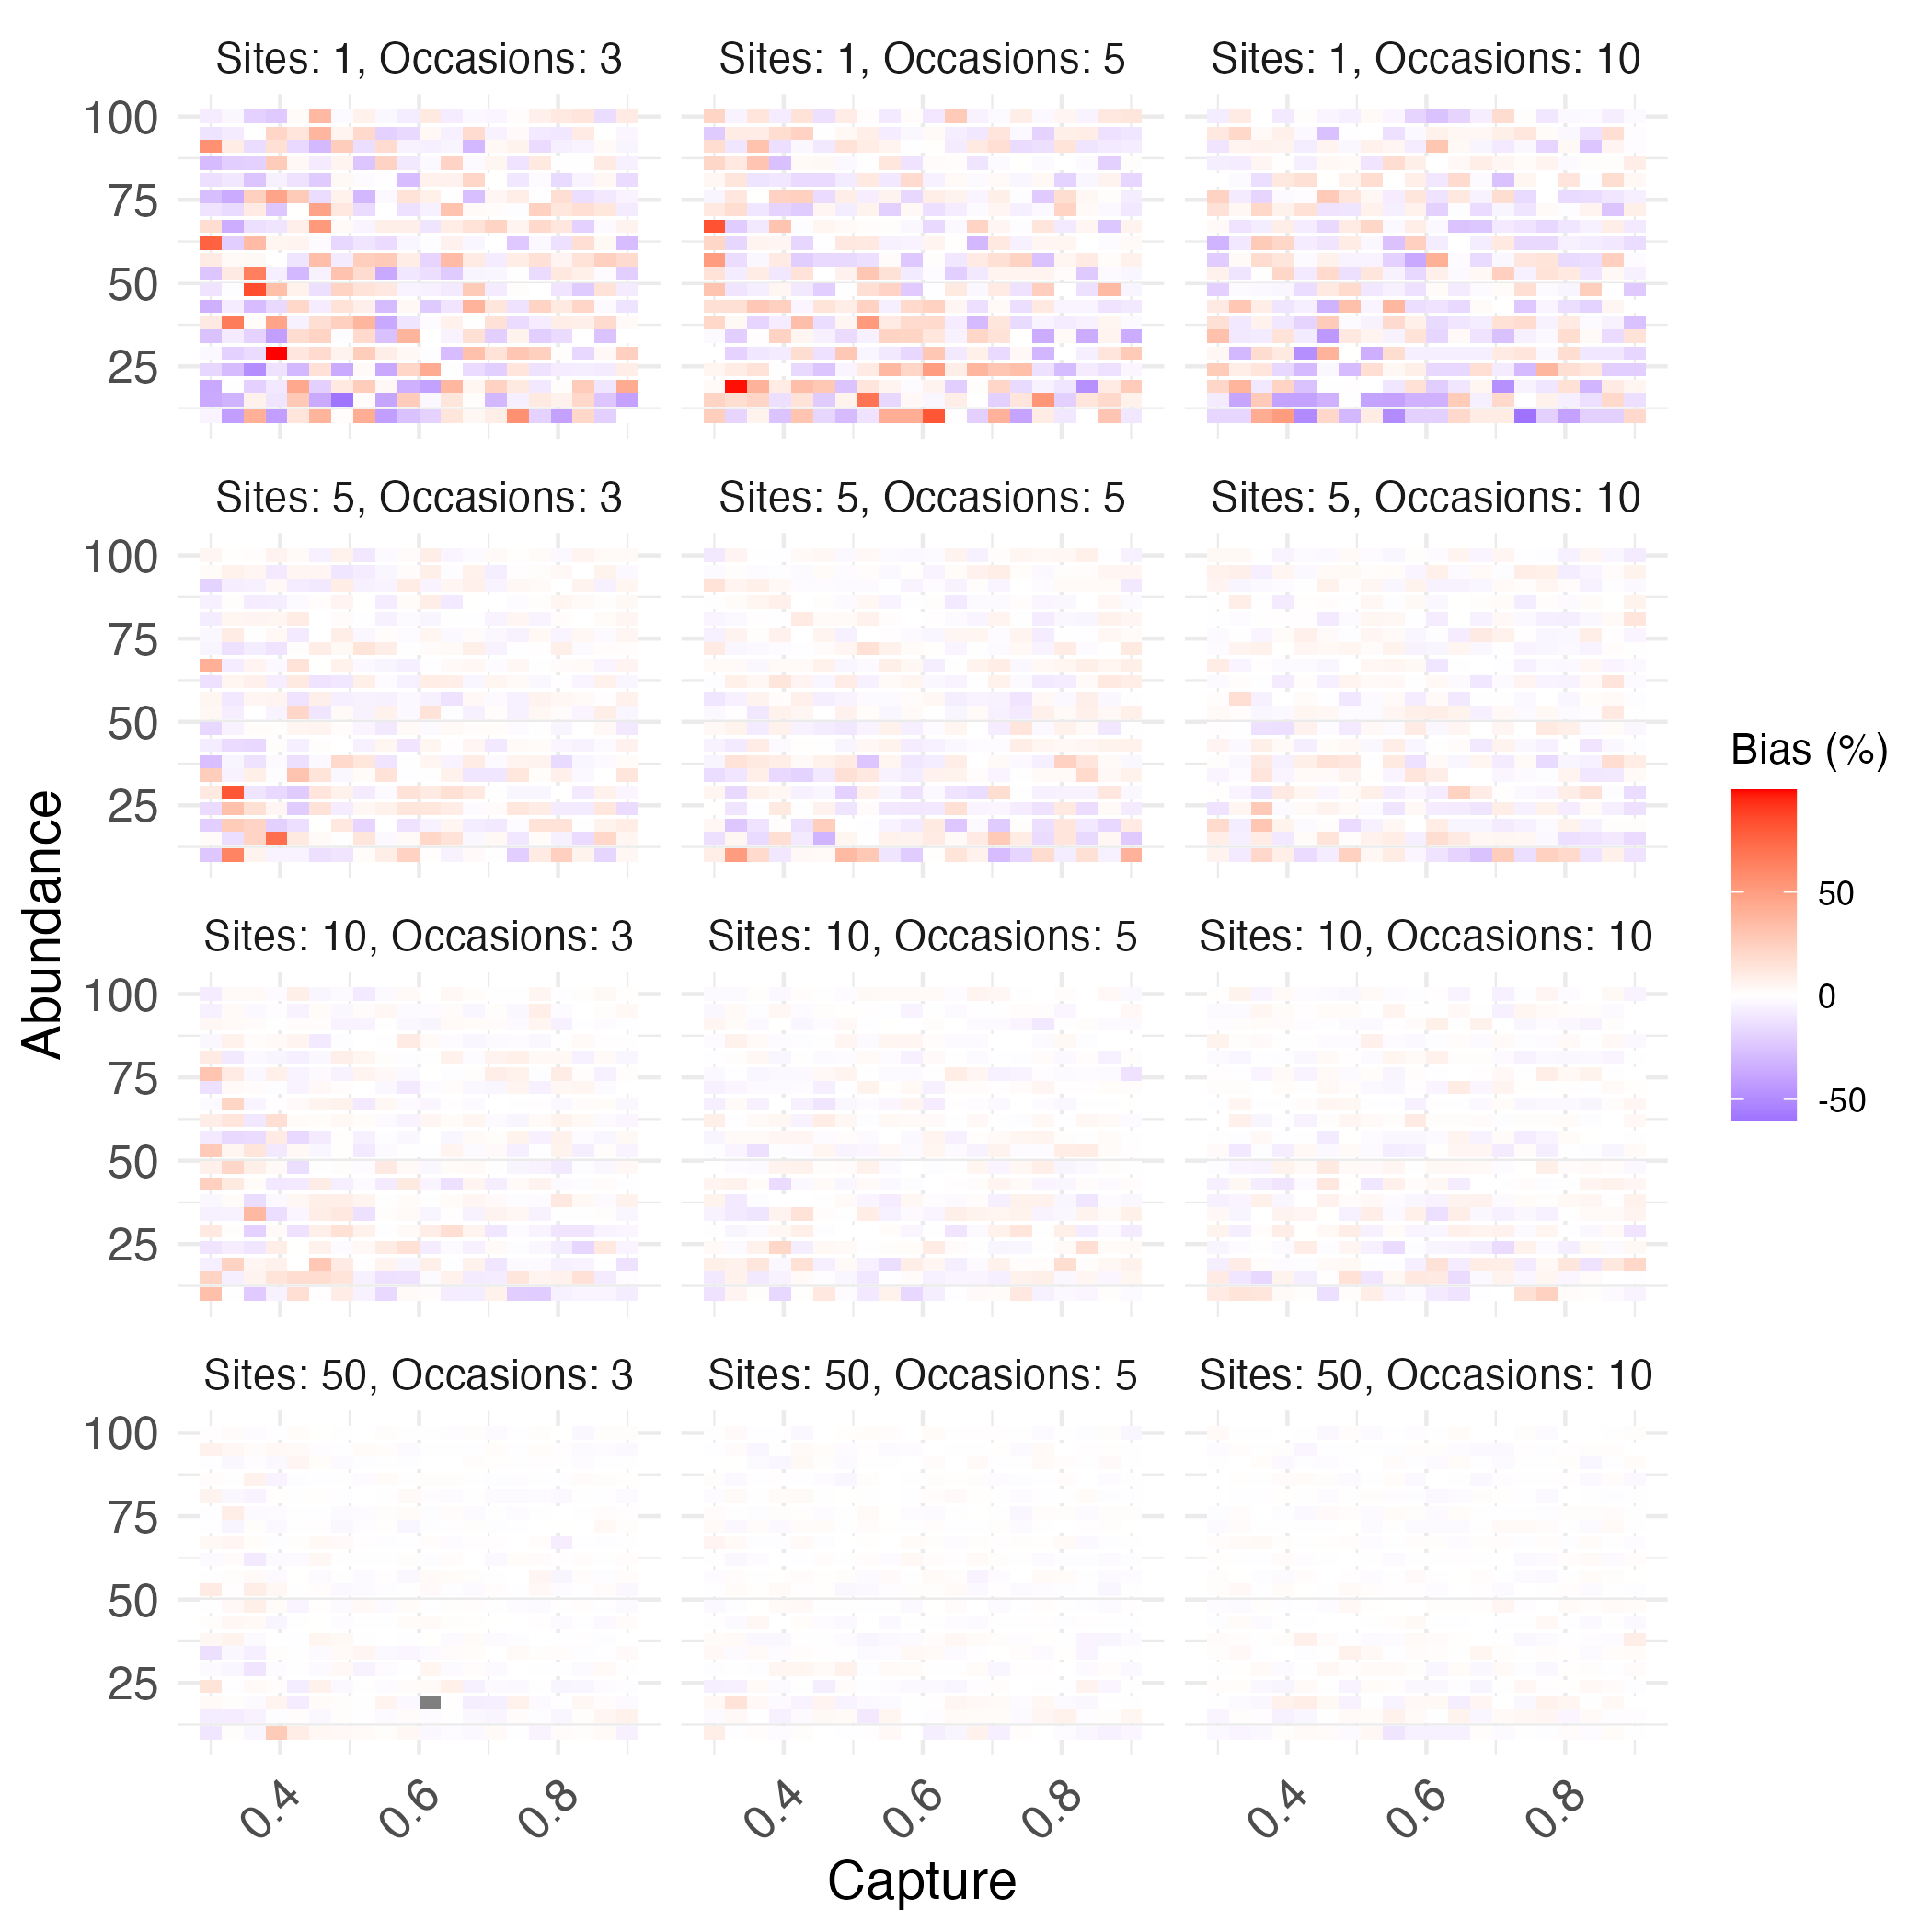
\includegraphics[width=0.98\linewidth]{heatmap_bias} 

}

\caption{Relative bias.}\label{fig:bias}
\end{figure}

\clearpage

\newpage

\begin{figure}[b]

{\centering 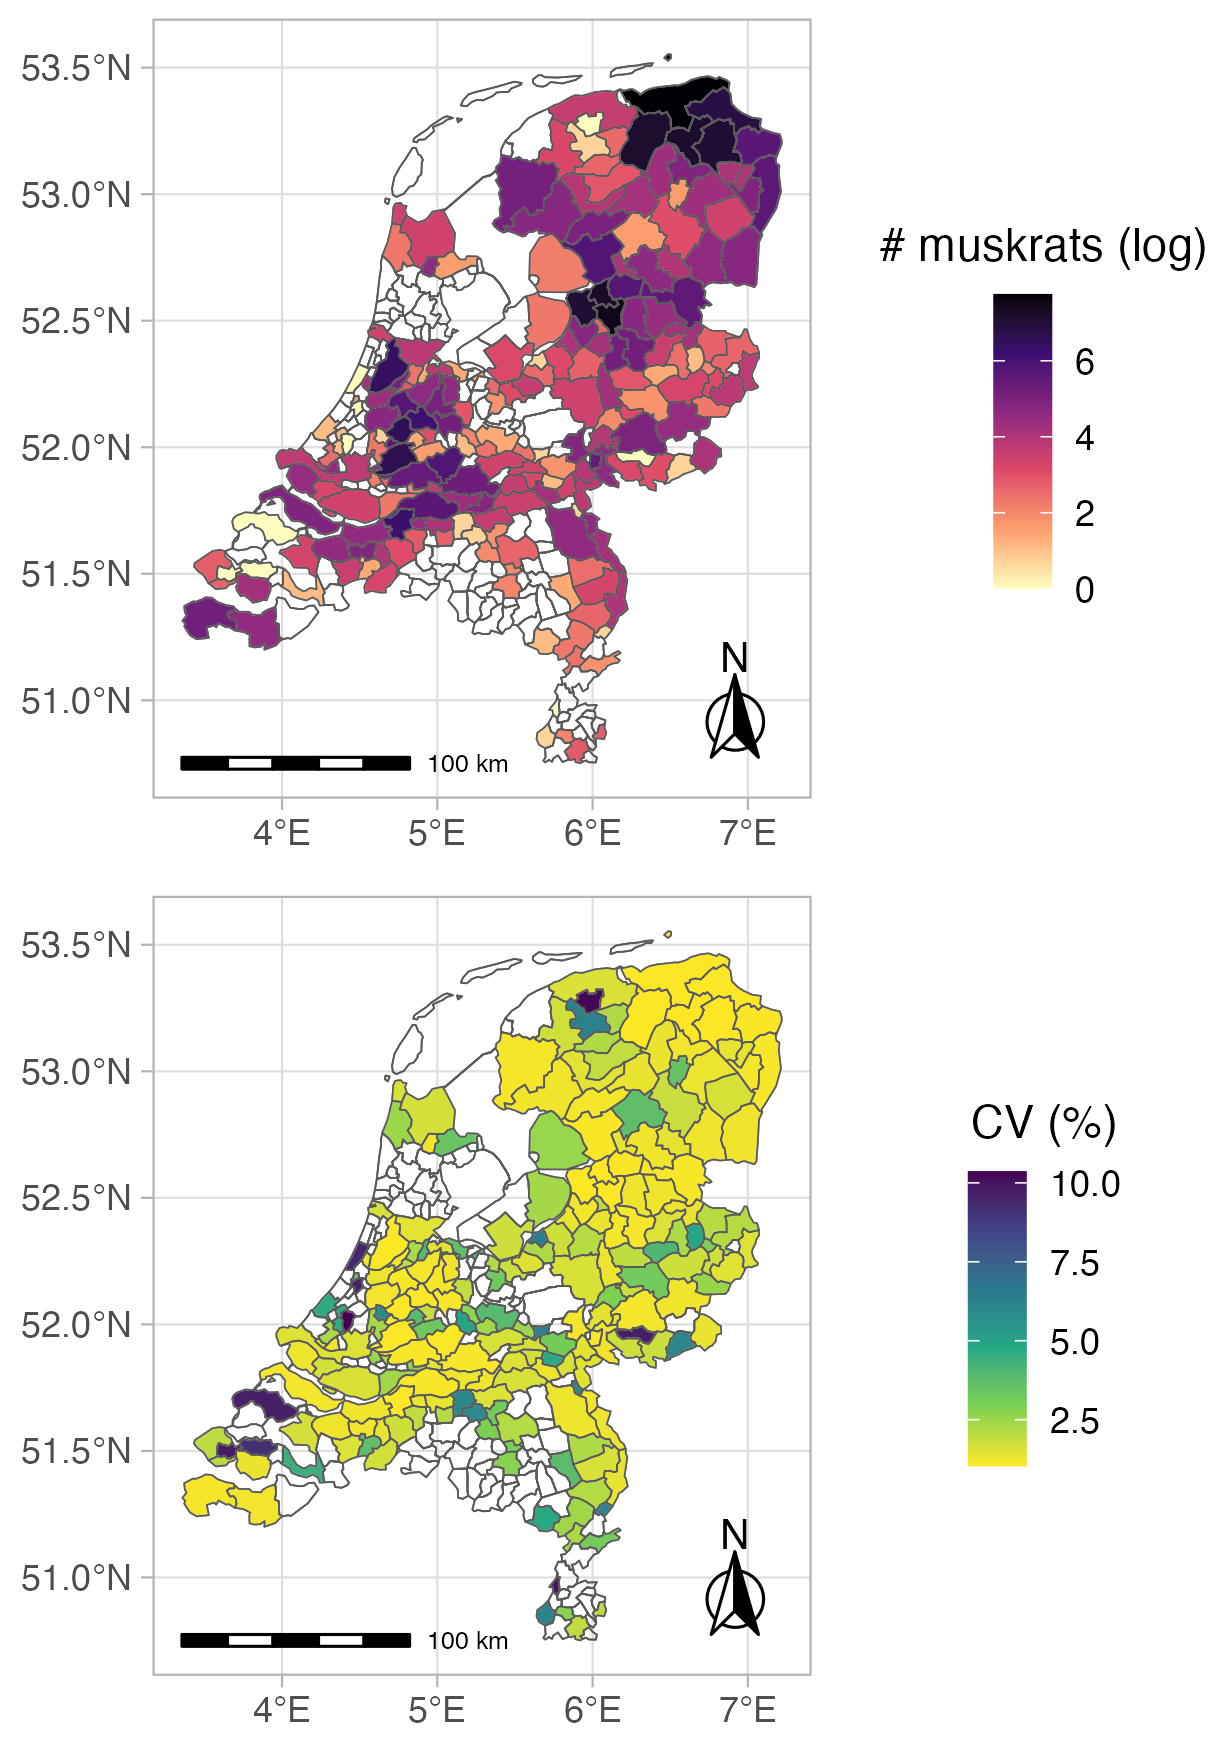
\includegraphics[width=0.95\linewidth]{muskrats} 

}

\caption{Muskrats.}\label{fig:muskrats}
\end{figure}

\end{document}
